% Funciones de activación y sus derivadas (2×2 groupplot)
% Compilar con: pdflatex activation_functions.tex
\documentclass[border=10pt]{standalone}
\usepackage{pgfplots}
\pgfplotsset{compat=1.18}
\usepgfplotslibrary{groupplots}

\definecolor{gdlblue}{RGB}{41, 98, 168}
\definecolor{gdlred}{RGB}{191, 49, 49}
\definecolor{gdlgreen}{RGB}{30, 130, 76}
\definecolor{gdlorange}{RGB}{217, 130, 30}
\definecolor{gdlpurple}{RGB}{118, 56, 138}
\definecolor{gdlgray}{RGB}{140, 140, 140}
\definecolor{gdlyellow}{RGB}{190, 140, 10}

\begin{document}
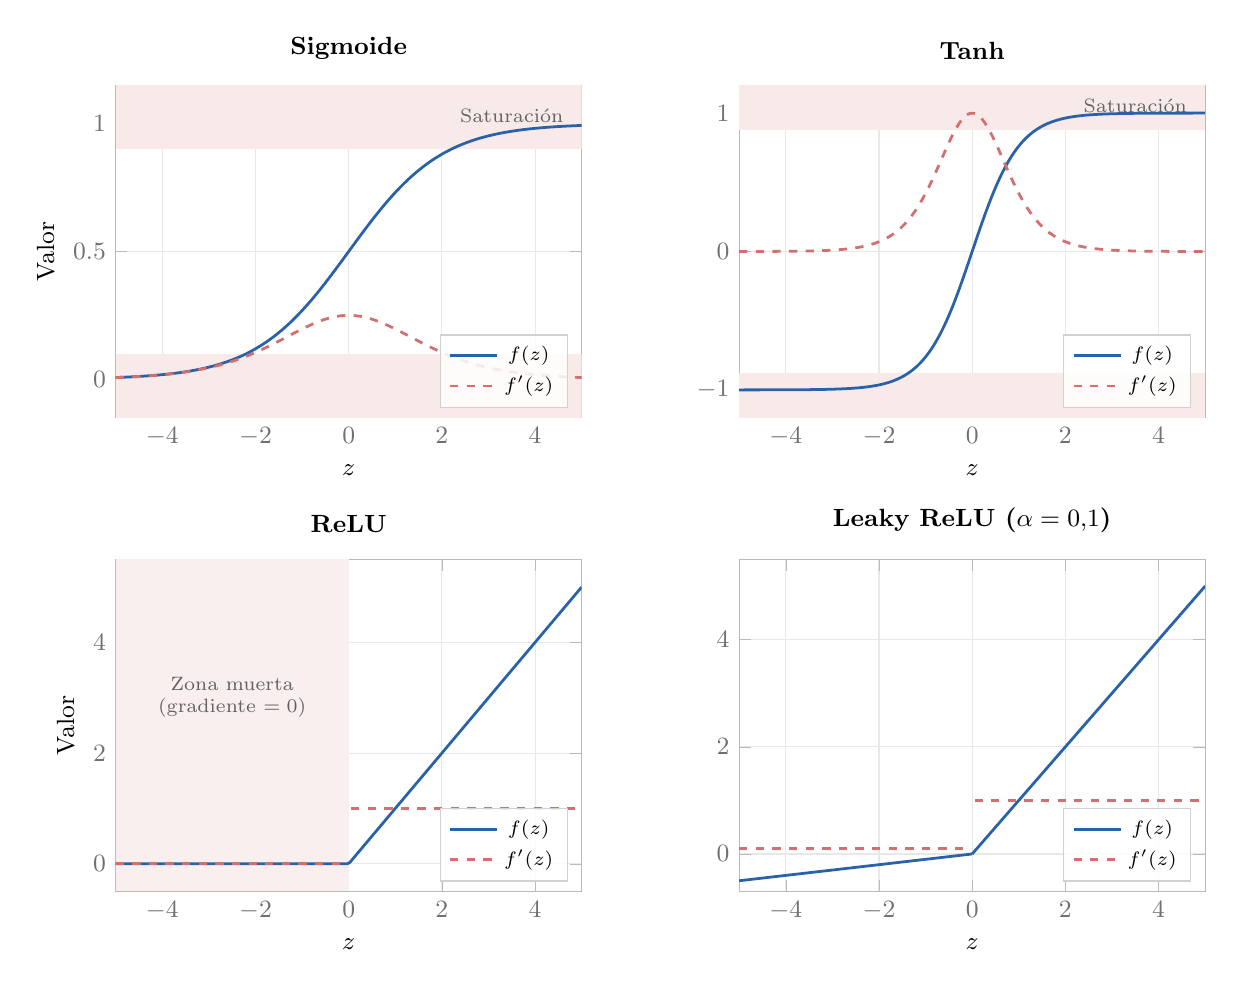
\begin{tikzpicture}
\begin{groupplot}[
    group style={
        group size=2 by 2,
        horizontal sep=2cm,
        vertical sep=1.8cm,
    },
    width=7.5cm,
    height=5.8cm,
    xmin=-5, xmax=5,
    xlabel={$z$},
    grid=major,
    grid style={gdlgray!20},
    axis line style={gdlgray!60},
    tick style={gdlgray!60},
    tick label style={font=\small, color=gdlgray!80!black},
    label style={font=\small},
    title style={font=\small\bfseries},
    legend style={
        font=\scriptsize,
        at={(0.97,0.03)},
        anchor=south east,
        draw=gdlgray!40,
        fill=white,
        fill opacity=0.85,
        text opacity=1,
    },
    every axis plot/.append style={line width=1pt},
    samples=200,
    domain=-5:5,
]

% ────────────── Sigmoide ──────────────
\nextgroupplot[
    title={Sigmoide},
    ymin=-0.15, ymax=1.15,
    ylabel={Valor},
]
% Zonas de saturación
\fill[gdlred!10] (axis cs:-5,0.9) rectangle (axis cs:5,1.15);
\fill[gdlred!10] (axis cs:-5,-0.15) rectangle (axis cs:5,0.1);
% Función y derivada
\addplot[gdlblue] {1/(1+exp(-x))};
\addlegendentry{$f(z)$}
\addplot[gdlred!70, dashed] {exp(-x)/(1+exp(-x))^2};
\addlegendentry{$f'(z)$}
\node[font=\scriptsize, text=gdlgray!70!black] at (axis cs:3.5,1.03) {Saturaci\'{o}n};

% ────────────── Tanh ──────────────
\nextgroupplot[
    title={Tanh},
    ymin=-1.2, ymax=1.2,
]
% Zonas de saturación
\fill[gdlred!10] (axis cs:-5,0.88) rectangle (axis cs:5,1.2);
\fill[gdlred!10] (axis cs:-5,-1.2) rectangle (axis cs:5,-0.88);
% Función y derivada
\addplot[gdlblue] {tanh(x)};
\addlegendentry{$f(z)$}
\addplot[gdlred!70, dashed] {1-tanh(x)^2};
\addlegendentry{$f'(z)$}
\node[font=\scriptsize, text=gdlgray!70!black] at (axis cs:3.5,1.05) {Saturaci\'{o}n};

% ────────────── ReLU ──────────────
\nextgroupplot[
    title={ReLU},
    ymin=-0.5, ymax=5.5,
    ylabel={Valor},
]
% Zona muerta
\fill[gdlred!8] (axis cs:-5,-0.5) rectangle (axis cs:0,5.5);
% Función
\addplot[gdlblue] {max(0,x)};
\addlegendentry{$f(z)$}
% Derivada (dos segmentos)
\addplot[gdlred!70, dashed, domain=-5:-0.05, samples=2] {0};
\addlegendentry{$f'(z)$}
\addplot[gdlred!70, dashed, domain=0.05:5, samples=2, forget plot] {1};
\node[font=\scriptsize, text=gdlgray!70!black, align=center]
    at (axis cs:-2.5,3) {Zona muerta\\(gradiente $= 0$)};

% ────────────── Leaky ReLU ──────────────
\nextgroupplot[
    title={Leaky ReLU ($\alpha = 0{,}1$)},
    ymin=-0.7, ymax=5.5,
]
% Función (dos segmentos)
\addplot[gdlblue, domain=-5:0, samples=2] {0.1*x};
\addlegendentry{$f(z)$}
\addplot[gdlblue, domain=0:5, samples=2, forget plot] {x};
% Derivada (dos segmentos)
\addplot[gdlred!70, dashed, domain=-5:-0.05, samples=2] {0.1};
\addlegendentry{$f'(z)$}
\addplot[gdlred!70, dashed, domain=0.05:5, samples=2, forget plot] {1};

\end{groupplot}
\end{tikzpicture}
\end{document}
